
\documentclass{article}
\usepackage[utf8]{inputenc}
\usepackage{graphicx}
\title{mlp3}
\author{ }
\date{February 2022}

\begin{document}

\maketitle

\section{Introduction}
\subsection{Motivation}
With the development of information technology, more and more digital images are available on the internet. Users often use various tags to describe the contents of their photographs when they share them. Accurate categorisation of these images and tags can better portray community images, facilitate the growth of user groups, increase commercial interest and benefit media research \cite{chua2009nus}.

\subsection{Literature review}


\subsection{Research Questions and Project Objectives}
There is often more than one feature information in an image and it is vital to be able to extract them accurately and comprehensively. We try to use the attention model as a baseline model and improve it to better accomplish multitasks and make predictions for multiple concepts of each image.
 
\subsection{Dataset and Task}
We used the dataset from the Lab for Media Search of the National University of Singapore \footnote{https://lms.comp.nus.edu.sg/wp-content/uploads/2019/research/nuswide/NUS-WIDE.html}. This dataset contains:
\begin{itemize}
\item[*] 269,648 images collected from Flickr, each image is around 24k in size;
\item[*] 81 concepts of groundtruth for evaluation and their corresponding label files;
\item[*] 64-D colour histogram, 144-D colour correlogram, 73-D edge direction histogram, 128-D wavelet texture, 225-D block-wise colour moments, and 500-D bag of words based on SIFT descriptions are six types of low-level features retrieved from these images.
\end{itemize}

The classification is multitasking, which means for each image, there is more than one label. We checked the number of images corresponding to each labels in the training set. The most is sky with 36,517; the least is map with only 33. The largest number of labels in training set are listed as in Table 1:

\begin{table}[t]
\begin{tabular}{llllllll}\hline
sky & 36517 & mountain & 2531 & horses & 900 & dancing & 393 \\
clouds & 26929 & boats & 2057 & leaf & 899 & protest & 384 \\
person & 23289 & nighttime & 2005 & fish & 873 & tiger & 351 \\
water & 17391 & house & 1924 & coral & 841 & fox & 333 \\
animal & 17141 & valley & 1907 & temple & 833 & waterfall & 299 \\
grass & 11176 & birds & 1905 & cars & 763 & castle & 266 \\
buildings & 8732 & sun & 1794 & sports & 750 & glacier & 252 \\
window & 7303 & military & 1568 & sign & 744 & harbor & 247 \\
plants & 7186 & garden & 1487 & police & 675 & computer & 246 \\
lake & 6715 & toy & 1386 & bear & 651 & swimmers & 220 \\
ocean & 5655 & food & 1327 & wedding & 603 & running & 206 \\
road & 4617 & plane & 1326 & frost & 565 & rainbow & 201 \\
flowers & 4290 & tower & 1276 & fire & 548 & whales & 192 \\
sunset & 4269 & dog & 1222 & statue & 493 & flags & 171 \\
reflection & 4023 & cat & 1208 & railroad & 488 & zebra & 162 \\
rocks & 3135 & street & 1199 & moon & 482 & book & 157 \\
vehicle & 2901 & bridge & 1170 & train & 451 & tattoo & 157 \\
tree & 2725 & town & 1162 & airport & 443 & surf & 97 \\
snow & 2655 & cityscape & 1108 & elk & 419 & soccer & 84 \\
beach & 2588 & sand & 1028 & cow & 398 & earthquake & 36 \\
 &  &  &  &  &  & map & 33 \\\hline
\end{tabular}
\end{table}
In addition we generated a matrix of $81*81$ to examine the relevance of the labels, as shown in Appendix. 

\subsection{Methods}
\subsubsection{Model Overview}
The model combines the research into image captioning completed in the Show, Attend and Tell paper with standard strategies for multi-label classification \cite{xu2016show}. The model first passes the 3 dimensional RGB channel through a convolutional block with an RELU activation. To support identification of the rotation invariant features max pooling is used to identify the most prominent image patches. From here a basic block is utilized for more feature segmentation which consists of 2 convolutional layers, activated by RELU functions. 
\newline
\newline
Following this initial feature extraction the data is passed through an attention layer. The key features of the data are identified by passing a further convolutions block through a maxpooling. This is then activated by a Softmax function to identify the relationship, or dependencies between the image features \cite{wang2017residual}. In parallel to this attention mechanism the data is fed through 2 convolutions blocks with the output of the attention layer being: $(1 + SMAX(X))*CONV(X)$. The output of this attention block is a vector that has captured both the principal features of an image and the relationship between the features. 
\newline
\newline
The attention block is fed through a residual block where the convolution space is reduced from 64 to 32 channels. The residual layer helps to reduce the likelihood of vanishing gradient and ensure important information is propagated through to the final activation layer. As the model (as it stands) is 32 layers strategies to reduce the likelihood of vanishing/exploding gradient are appropriate. The reduction of feature layers is completed to capture non-linear relationships between the features and the labels. The final steps are creating a flat, 27 dimensional vector that is activated using the Sigmoid function. Sigmoid is chosen as an activation function because we're trying to capture the independent probability of each independent label, so is an appropriate activation function for binary-cross entropy which is used to determine the efficacy of the model.
\newline
\newline
Figure one contains a diagram of the model, and a full summary is included in the appendix:
\newline
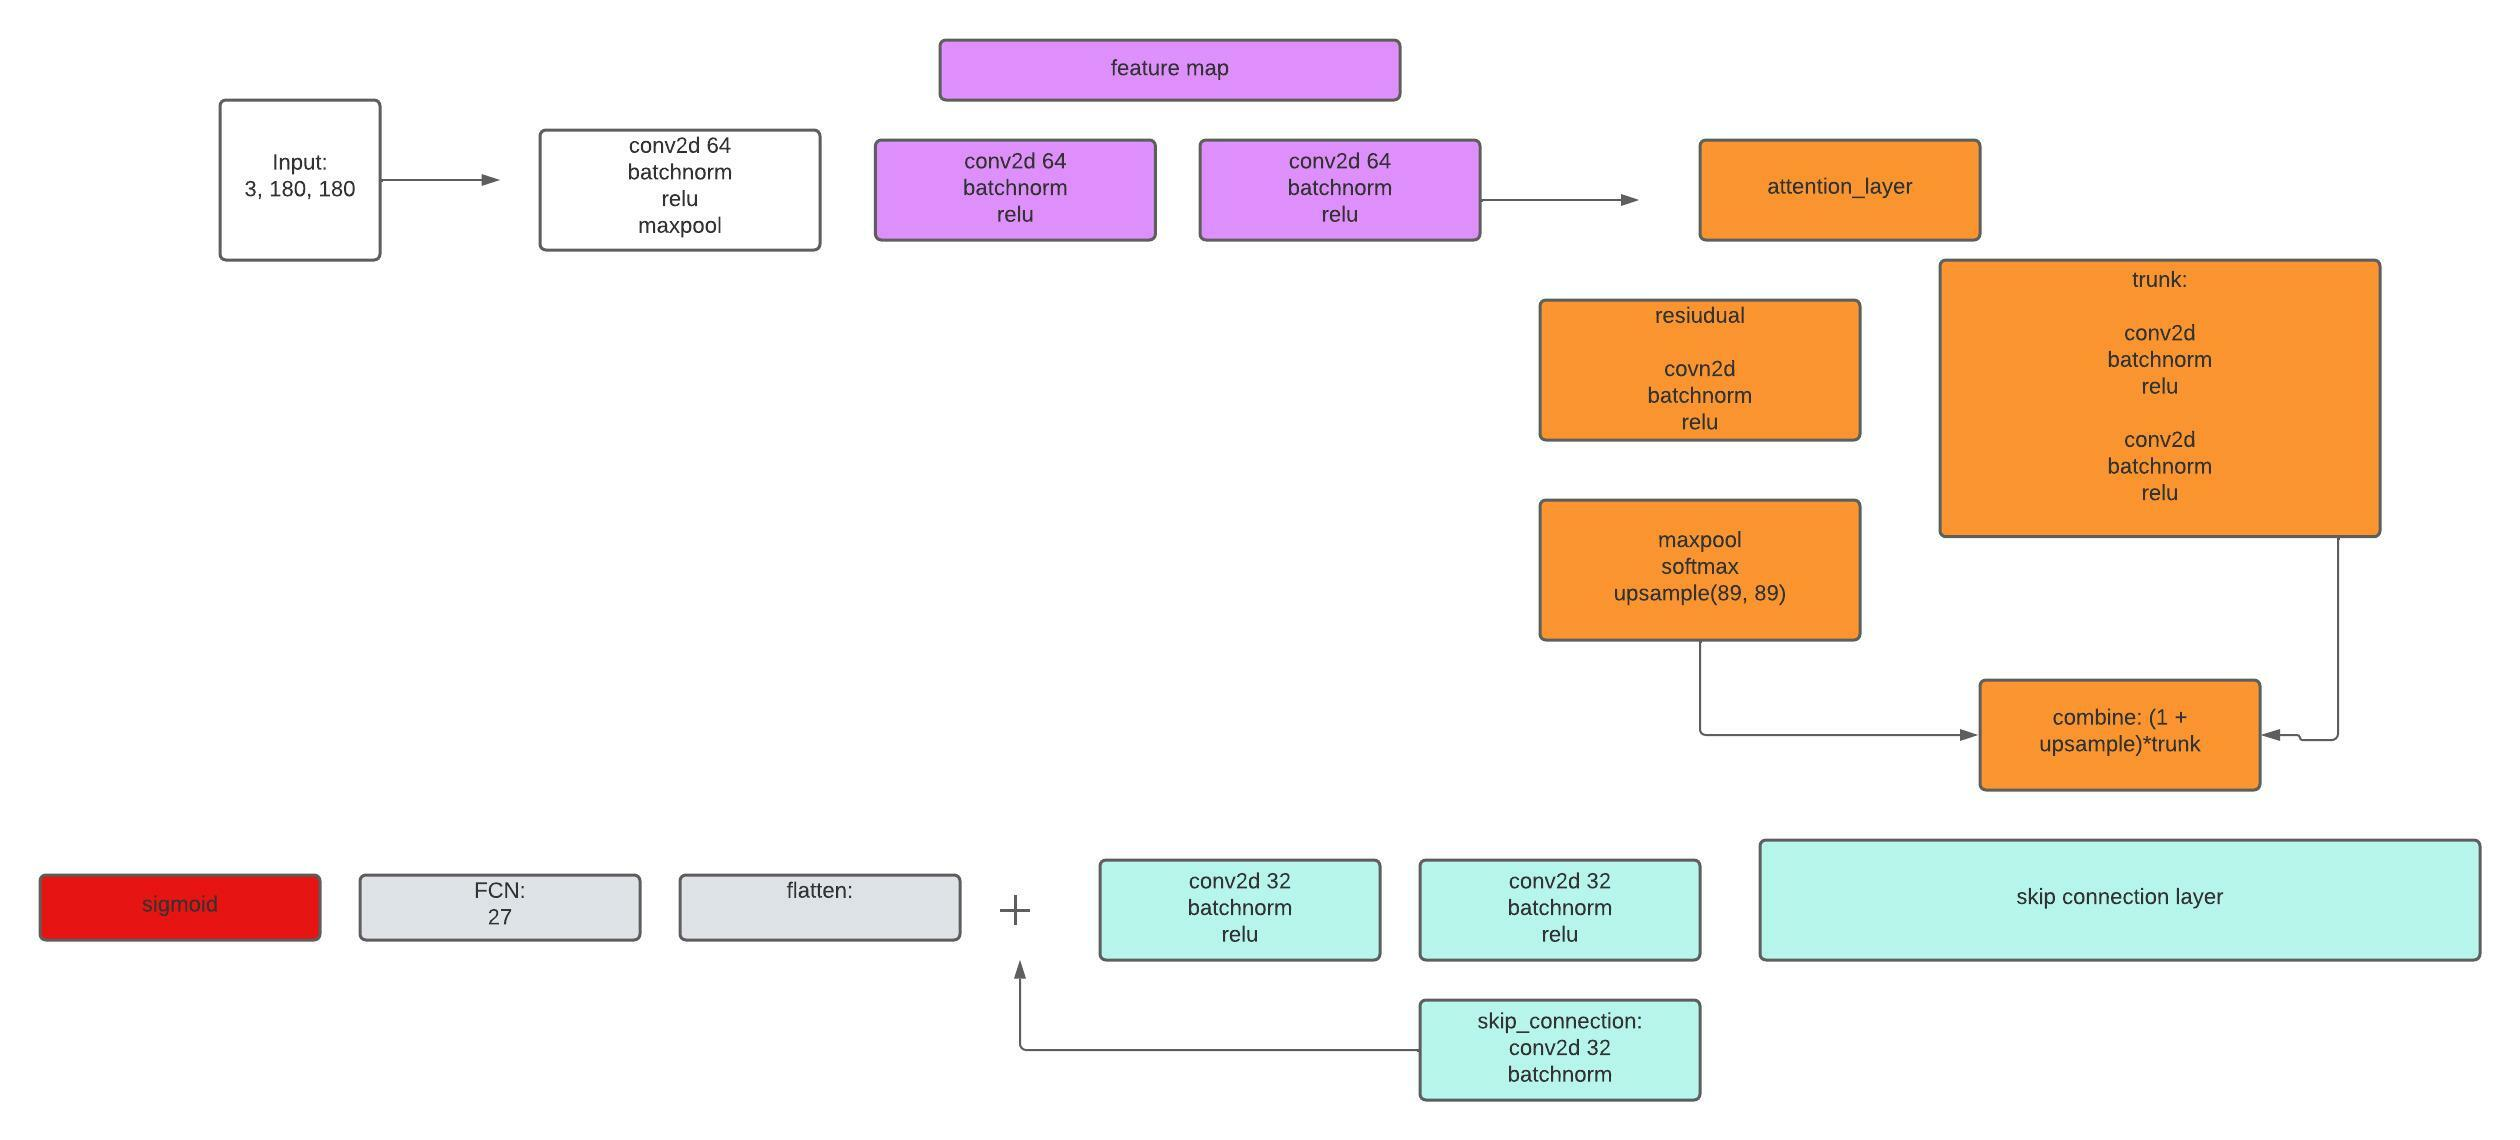
\includegraphics[scale=0.3]{attention_uml_v1.jpeg}
\subsection{Baseline Experiments}
The model was trained (initially) on a small subset of the training data. The training dataset was iterated over 35 times with back-propagation ran to support identification of model parameters to minimize the associated error with each label. 
\newline
\newline
The mean precision, error, F1 and binary cross-entropy are plotted in the figures below. The divergence in performance between the training and test dataset is typical of overfitting, where the model identifies parameters that reflect biases in the training dataset that do not extend to the overall population. 
\newline
\newline
The mean error, accuracy (both in terms of precision and recall) are plotted in the figures below. The fast convergence demonstrate that the attention model, as it stands, has a high propensity to overfit the data (no evaluation has been completed of the test dataset as of yet). To address this strategies to reduce over-fitting such as dropout and regularization will be implemented to support generalization to the test dataset. As part of improving the performance of the model we will also look at data augmentation and under what combination of labels the model performs well to develop a data augmentation strategy to address data imbalance and distribution issues. Finally, we will compare running the model with and without the attention model to explore what role it's playing in the model performance and look at visualizing the components/features identified by the attention module to see if it's aligned with the capabilities identified in the show, attend and tell paper. 
\newline
\includegraphics[scale=0.3]{results_small_v1.png}
\subsection{Interim conclusions}
We used the attention model to train the NUS dataset, which contains the network images and their corresponding 81 labels in total. The difficulty in this problem lies in multitasking, e.g. an image corresponding to both the label sky cloud etc. We have currently used a small part of the dataset and have experienced overfitting. In the next step, we will expand the use of the dataset and add algorithms such as dropout to solve the overfitting. In addition, we will further investigate the issue of label correlation in the dataset to develop a better way to fit the dataset.
We either adopt the recurrent attention CNN approach, i.e. introduce an attention mechanism in machine learning to improve the accuracy of multi-tasking in network learning by recursively analysing local information and thus extracting the necessary features.
%%• Plan for the remainder of the project, including discussion of risks, backup plans
\subsection{Appendix}
\subsubsection{Model Summary}
\includegraphics[scale=0.7]{model_summary.png}
\subsubsection{Data Correlation}

\end{document}
